\chapter{Accessing Knowledge}
\section{Search Strategies}
The task of knowledge sharing between different disciplines of the scientific or engineering realm can be difficult to achieve with precision and reliability. To ensure those, one possibility is to rely on function-based solutions. Here, it is important to specify that functions are not intended in the mathematical sense, but rather refer to the purpose of a thing - or, to say it more simply, to whatever it is used for. Being the priority of customers, function plays a fundamental role in business. To bring it to a practical level, the shift between selling washing powder and selling cleaned clothes, representative of the function of the first, most certainly will increase the sales of the washing powder company that has the intuition of presenting itself this way to the market. The combination of this shift with a re-arrangement in term of functions of the knowledge databases is a huge step. To accomplish that, Mann suggests an organization by function words of the databases and search in the business context. Here, the focus should be moved from nouns to verbs. When thinking about something, in fact, the first thought normally goes to \textit{things}: people, objects, companies, etcetera. However, it is the \textit{connection} between the things that allows to put them right into their place. This connection is expressed by the verbs, or, to put it in a more technical language, the predicates in the subject-predicate-object triple. That the focus should lie on verbs rather than nouns is made clear by the will of expressing relationships. If we stick to semantics rather than diving into the field of informatics, \textit{predicates} of a sentence are the verbs, whereas \textit{subject} and \textit{object} are normally expressed by nouns. In addition to this focus on verbs, Mann also offers a categorization and selection of \textit{function verbs}. They are grouped as follows:
\begin{itemize}
    \item Accomplishment verbs
    \item Creative verbs
    \item Clerical or detail verbs
    \item Communication verbs
    \item Financial verbs 
    \item Helping verbs
    \item Management verbs
    \item Research verbs
    \item Technical verbs
    \item Negative verbs.
\end{itemize} \\
\\
\subsection{Differences with the ER-Model}
A few critical aspects can be found in Mann's proposal for a function-based organization of databases. He writes of "things", which, however, are not better defined. How classes of things should be treated and what the approach to multiple applicability of a single function should be thus remain open questions. However, it is important to remember that Mann's proposal does not claim to be technical, but rather approaches the problem from the business point of view. One technical proposal for a data model that covers the above mentioned points and presents some important similarities with Mann's functional model is the well-known Entity-Relationship Model, first described in 1976 by Peter Chen \cite{che76}. Due to its technical purpose and its higher level of accuracy, Chen's model obviously presents some huge differences with Mann's proposal and investigates more deeply some aspects that are neglected by Mann. Therefore, the absence of \textit{attributes} and \textit{values}, present in [Che76], is not only ascribable to Mann's focus on verbs and verbs only as function expressions, but also to a broader, less precise view of the problem - the same reason why Chen's Entity Sets and Relationship Sets do not find their homologous in Mann's proposal, and the problem of multiple applicability of relationship is not even mentioned. 
\begin{figure}
	\centering
	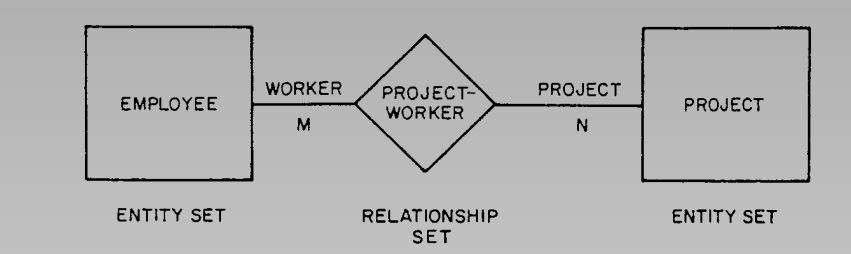
\includegraphics[width=\textwidth]{pic2.png}
	\caption{Example of a simple Entity-Relationship diagram. \cite{che76}}
\end{figure}

Apart from these technical differences, the two proposals seem to lie on a common ground - strangely enough, since Mann does not even mention Chen's well-known and way older model. However, the main difference seems to lie in the interpretation of \textit{relationship}. Mann confines them to verbs, whereas in the ER-Model they are often expressed by other nouns (e. g. "worker"). Moreover, according to Mann's proposal the chosen verbs should belong to specific categories and only refer to the \textit{function} of the entity to specify. In order to understand this, it has once again to be taken into account that Mann's proposal is only directed to \textit{business} models, whereas the ER-Model should be apt to describe every possible database. Proposals for an ER approach to knowledge bases had already been done, like the one by Karukonda, which aims at proposing an unified ER-based framework for knowledge based systems \cite{karukonda}. It is evident that the difference between those approaches and Mann's proposal lies in the central role of functions and the precise classification of the verbs that should express them is a further support to this argumentation. Nevertheless, the critical aspect of Mann's proposal remains that the databases that lie at the bottom of a business model can be of any kind - therefore, a model that only includes some can be seen as incomplete, and the hypothesis that any database could be seen in terms of functions and its relationship expressed with verbs is arguable. The question that arises is if a database of no apparent interest for business should be ignored - since it is not relevant for business models - or transformed in terms of functions, in the case that it could be present in a database e. g. of a company.\\
\\
If a function-oriented organization of databases still presents some difficulties, a function-oriented search strategy as proposed by Mann lays the foundation for obtaining relevant results - at least in the business sector. \newpage
\section{Knowledge Search Tools}
Strategies for an useful search are indeed helpful, but their value increases a lot when they are supported by search tools or engines which facilitate the work. 
When searching for something, the user aspires at finding the highest amount of information in the lowest possible amount of time. Resolving this time-versus-content conundrum should be a priority of smart business companies.\\
\begin{figure}[h]
	\centering
	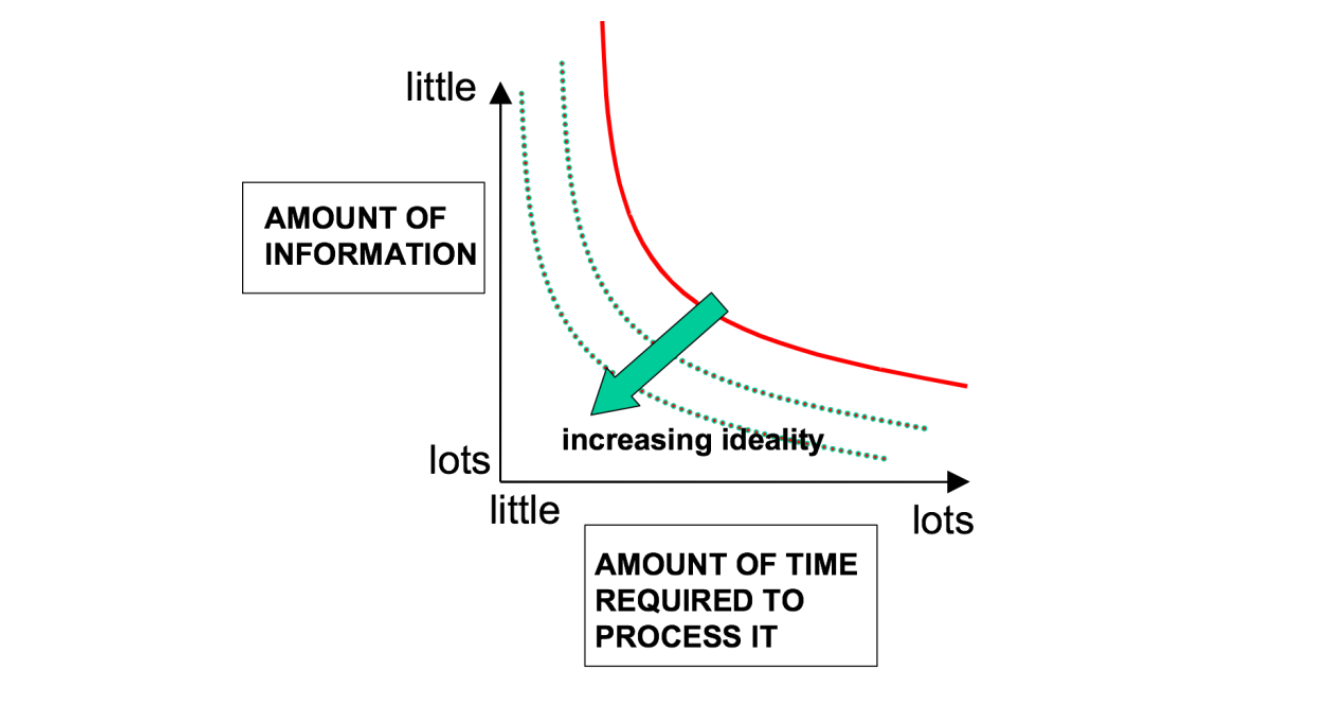
\includegraphics[width=\textwidth]{pic3.png}
	\caption{The time-versus-content conflict. \cite{darrell2004hands}}
\end{figure}\\
It could also be argued that finding the highest possible amount of information is not always useful; on the contrary, it may even become counterproductive. More than quantity, it is quality that a search result should provide. Getting 5 relevant results is better than getting 500 results - which will contain the relevant ones, but also some rubbish. However, this is a contradictory section of Mann's book, because the tools that are listed as useful for finding a solution to the time-versus-content conflict actually focus on providing the most relevant results - a feature that Mann himself points out. The mentioned tools are the following:
\begin{itemize}
    \item Search Engines
    \item Semantic Search Tools
    \item User-Defined Context Search Tools
    \item Intelligent Agent-Based Search Tools.
\end{itemize}
Even though they may return a huge amount of results, it is probably already clear that the feature they present - e.g. the ability of providing context - aim at precision and relevancy rather than quantity. In the next paragraphs, these tools will be presented individually according to Mann's description.
\subsection{Search Engines}
Among the most important search engines is, of course, Google. It is known to everyone who has ever surfed the Internet that Google provides quick and relevant results - in fact, the answer to our query will probably lie among the first 10 results. If Google were to be considered according to Figure 2.2, it would most certainly score a high ideality value, since it provides a huge amount of results in a few seconds. Google is also a demonstration of the fact that a huge amount of results is not necessarily confusing. However, understanding the functioning of Google can make the research more effective. Google is based on keyword, but it also takes into account the distance between the words. For example, a query for motivational techniques in service industry contexts may be googled with a string like "motivation service industry". After identifying all the documents that contain this string, Google will sort them by priority according to how close together the input words are.
\subsection{Semantic Search Tools}
Semantic Search Tools are built on the subject-action-object concept of systematic innovation. They work by extracting the subject, action and object elements for every word in the search string. For example, a search like "reward staff" will return all the sentences in which "reward" is the action and "staff" the objects; It will also consider synonyms of both verbs. Moreover, it will extract the subject of the sentences - which represent the answer to the question "how can I reward my staff?".
\subsection{User Defined Context Search Tools}
While the two above mentioned kinds of search tools have the huge problem that they do not take the context of the search into account, this third category aims at solving this issue. At first, these tools were built around a knowledge classification system (like a taxonomy) or an ontology, thus forcing the user to pigeonhole information into a pre-defined knowledge structure. The main problematic of this approach is the difficulty of fitting a piece of information into a single category. Therefore, a certain degree of adaptivity was reached, in order to allow the information to move from one cell to another. These tools present some critical aspects. Since they rely on knowledge structures, in fact, the context that they guarantee is general and quite fixed - a much more useful context is the one provided by Intelligent Agent-Based Search Tools, as explained in the next paragraph.
\subsection{Intelligent Agent-Based Search Tools}
Intelligent Agent-Based Search Tools learn about the context by observing the user. An example could be Amazon: If you buy Shakespeare's \textit{Macbeth}, you will notice that Amazon will suggest you other Shakespearean works, and probably also other dramas of similar period or in the same language, or maybe other versions of the same tragedy. It is noticeable that this type of context is much different than the one that can be provided by knowledge structures - however adaptable they may be. Here, Mann's argumentation lacks a definition of a broad concept like context. Perhaps the purpose of this lack is to leave more possible interpretation of the term, in order to consider many different tools. In fact, the differentiation between context types is one fundamental aspect when dealing with search tools. Voskarides, for example, divides them into (1) context provided by the search tool or engine to enrich search results (e.g., by searching for a city it is very likely to find information about tourist attractions), (2) context originated from interactions between the user and the search machine, and (3) context provided by the user to specify a broad query. \cite{voskarides} Interestingly enough, Voskarides does not pay much attention neither to the context that the machine learns by observing the user - although it is partly covered by the chapter on conversational search - nor to the context that can be derived from a knowledge structure.
\\
Once again, it is important to remember that Mann's book does not cover many technical aspects due to its business-oriented perspective. One important point that he does not consider regards the different approach to different way of storing knowledge. As Voskarides points out, knowledge can be structured - e.g. in form of a knowledge graph - or unstructured - e.g. textual data or social media posts. \cite{voskarides} The structure of these underlying knowledge repositories is, of course, fundamental for search tools developers in order to enrich their offer. Knowing the different ways of knowledge storage is useful for the users of these search tools as well, in order to refine their search input. 
\newpage
\chapter{Knowledge and Wisdom}
This paper - and Mann's book chapter - has focused on knowledge access strategy without \textit{precisely} defining what knowledge is, but only relying on a broad - maybe even vague - understanding of the concept. Using a search engine allows to find data which may contain some useful information to answer our question. However, all these concepts - data, information, knowledge - despite being similar, are not synonyms and clearly cannot be used as such. 
In the third chapter of his book, Mann focuses on the shift from knowledge to wisdom, which he defines as follows:\\
\textit{Knowledge is when you know that tomato is a fruit; Wisdom is when you know not to put tomatoes in a fruit salad.} \cite{darrell2004hands}\\
Like in most studies on knowledge management, Mann relies on the DIKW (Data - Information - Knowledge - Wisdom) scheme, presented in Figure 3.1. Here, all the above mentioned concepts finally come into place. \\
\begin{figure}[h]
	\centering
	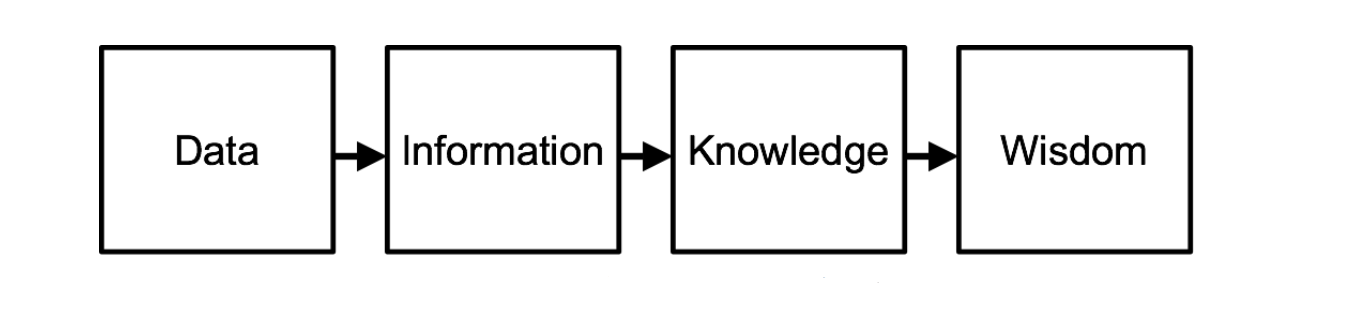
\includegraphics[width=\textwidth]{pic4.png}
	\caption{The DIKW scheme. \cite{darrell2004hands}}
\end{figure}\\
At this point, Mann takes for granted the understanding of this scheme, which requires some prior understanding - providing definitions is a difficult task, due to the overlapping of concepts and their abstractness. Even looking at the already provided definitions can be confusing, since they often differ. Another difficulty in understanding this scheme relies in its hierarchy: To define a concept, the subordinated ones are taken as paradigma. As explained by Baškarada and Koronios\cite{DIKW} and by Rowley\cite{DIKW2}, data are elementary, unorganised and unprocessed descriptions of things, without meaning, context or interpretation; Information is data - or an aggregation of it - shaped into a form meaningful to humans and useful; Knowledge is data and/or information organised and processed, to which are added understanding, expertise, and opinions; Wisdom is the highest level of abstraction, provided by accumulated knowledge, and allows to apply concepts from one domain to new situations or problems.\cite{DIKW}\\
\\
This definition of knowledge recalls TRIZ (Russian acronym
for “Teoria Reshenia Izobretatelskih Zadach”, "Theory of Inventive Problem Solving"), which can be applied to problem solving in different domains. \cite{TRIZ} Mann attributes a huge importance to the broadness of applicability of his theories - at least concerning business model. This could be a common ground with TRIZ, in which the abstraction of problems plays an important role. Another aspect of interest of TRIZ in relation to Mann's theories is that it provides a functional approach. 
\subsection{Function Analysis in TRIZ}
In TRIZ, Function Analysis is composed by 4 key stages.\cite{TrizManual}
\begin{itemize}
    \item \textbf{Component Analysis:} This step consist in the identification of the components of the analyzed systems. Also a supersystem is identified.
    \item \textbf{Interaction Analysis:} All possible interactions between the components and their supersystems are identified.
    \item \textbf{Function Modeling:} This step consists in the identification and evaluation of the functions performed by the components of the system and the supersystem.
    \item \textbf{Cost Analysis:} This step consists in the calculus of the absolute and relative costs of all components.
    \end{itemize}
Mann's proposal finds its corresponding step in Function Modeling, where all functions are identified. However, one important characteristic of Function Modeling in TRIZ is its \textit{divide et impera} approach. The first step of Function Analysis is, in fact, a component analysis. Moreover, the functionality of a system is delivered by the functionality of its single components. \cite{TrizManual} A car, for example, has the function of moving passengers and cargo, and its components - motor, brakes, etcetera - contribute to build this function. Mann does not mention the possibility of a subdivision of functions or of a hierarchical model. Here lies the huge difference between the function-based proposal by Mann and the Function Analysis in TRIZ. 
\newpage
\chapter{Knowledge Management}
Until now, strategies and tools for accessing knowledge were discussed. However, once the knowledge has been acquired, it is necessary to manage it. Knowledge Management is a problem with which scientists has dealt for the past decades - and it is remarkably comprehensive of every domain. Again, as for wisdom, the field becomes very difficult to adventure in, due to the fact that concepts overlap and are difficult to define - not to mention its multidisciplinarity. 
\\
Rather than defining the main features of a business model for knowledge management, Mann lists the common aspects of successful business models. First of all, he  mentions trust. Then, once trust is present, the faith in the power of self-organisation in systems is important - which leads to his third point: the absence of a knowledge organization department. This should be avoided in order to protect the business and not the knowledge \textit{per se}. Moreover, they would send the message that knowledge management is someone else's responsibility - whereas it should be overarching. This idea is supported by other authors as well. Dalkir, for examples, cites Gray and describes knowledge management in business contexts as "[...] a collaborative and integrated approach to the creation, capture, organization, access and use of an enterprise’s intellectual assets." \cite{KMTP} The adjectives \textit{collaborative} and \textit{integrated} here are fundamental: The management of knowledge has to be spread through all the sectors of a business system, and not concentrated in a single one.\\ \\ Last but not least, Mann cites the ability to forget knowledge that is no longer relevant. For example, a change of context would make the memory of old knowledge not only not useful, but even confusing. Therefore, being able to remove old knowledge is important. In this chapter, however, the presented theories are not further investigated - which leaves room for a lot of open questions. For example: How can the shift of knowledge from "useful" to "not useful" be recognized? Corporate memory, as Mann himself states in this chapter, is both a good and a bad thing. This implies that knowledge should not always be forgotten - only in the cases when it is "not useful (anymore)". 
